\documentclass[12pt,a4paper]{article}
\usepackage[utf8]{inputenc}
\usepackage{graphicx} 
\usepackage{minted}
\usepackage{ragged2e}
\usepackage[a4paper, left=0.5in, right=0.5in, top=0.5in, bottom=0.5in]{geometry}
\usepackage{minted}
\usepackage{rotating}
\usepackage{float}

\begin{document}

\begin{titlepage}

\begin{center}

\textup{\small {\bf EC3066D - ARTIFICIAL INTELLIGENCE: THEORY AND PRACTICE} } \\[0.2in]

% Title
\Large \textbf {Implementation of Algorithms} \\[0.4in]
\bf {Artificial Intelligence, Machine Learning and Deep Learning} \\[0.7in]

% Submitted by
\normalsize Submitted by \\
\begin{table}[h]
\centering
\begin{tabular}{lr}\hline \\
Roll No & Names of Students \\ \\ \hline
\\
Narendiran S & M190412EC \\
M.R.K Siva Naga Sai & M190413EC \\ 
Rahul Kumar & M190616EE \\
K. Sai Kiran & M190296EE \\ \\ \hline 
\end{tabular}
\end{table}

\vspace{.1in}
Course Faculty: Ms. Lyla B. Das/Mr. Sreeram M.\\[0.2in]

\vfill

% Bottom of the page

\includegraphics[width=0.18\textwidth]{{./images/nitc}}\\[0.1in]
\Large{DEPARTMENT OF ELECTRONICS AND COMMUNICATION ENGINEERING}\\
\normalsize
\textbf{NATIONAL INSTITUTE OF TECHNOLOGY, CALICUT-673601}\\

APRIL 2020

\end{center}

\end{titlepage}

\tableofcontents

\newpage
\section{IMPLEMENTATION OF MACHINE LEARNING ALGORITHMS}

\subsection{GRADIENT DESCENT}

\subsubsection{Aim}
\quad \quad To Implement Gradient Descent with different values of the Learning Parameter and show with help of a Simulated Figure, Convergence rates change.


\subsubsection{Description}

\quad \quad Optimization is a big part of machine learning. Almost every machine learning algorithm has an optimization algorithm at it’s core.

\quad Gradient descent is an optimization algorithm used to find the values of parameters (coefficients) of a function (f) that minimizes a cost function (cost). It is best used when the parameters cannot be calculated analytically (e.g. using linear algebra) and must be searched for by an optimization algorithm. 

\quad The procedure starts off with initial values for the coefficient or coefficients for the function. These could be 0.0 or a small random value. 
\begin{center}
Co-efficient = 0.0 
\end{center}

\quad The cost of the coefficients is evaluated by plugging them into the function and calculating the cost. 
\begin{center}
cost = f(coefficient)       or           cost = evaluate(f(coefficient)) 
\end{center}

\quad The derivative of the cost is calculated. The derivative is a concept from calculus and refers to the slope of the function at a given point. We need to know the slope so that we know the direction (sign) to move the coefficient values in order to get a lower cost on the next iteration. 
\begin{center}
delta = derivative(cost) 
\end{center}

\quad Now that we know from the derivative which direction is downhill, we can now update the coefficient values. A learning rate parameter (alpha) must be specified that controls how much the coefficients can change on each update. 
\begin{center}
coefficient = coefficient – (alpha * delta) 
\end{center}

\quad This process is repeated until the cost of the coefficients (cost) is 0.0 or close enough to zero to be good enough. 

\quad You can see how simple gradient descent is. It does require you to know the gradient of your cost function or the function you are optimizing, but besides that, it’s very straightforward 


\subsubsection{Dataset used}
\quad \quad The dataset used consist of 100 data points and two features. The two features are exam scores in two different subject. The output variable is either 0 or 1 representing Not Getting Admitted or Getting Admitted.
\subsubsection{Methodology To Implement This Algorithm}

\quad \quad Gradient descent is a generic optimization algorithm used in many machine learning algorithms. It iteratively tweaks the parameters of the model in order to minimize the cost function. The steps of gradient descent is outlined below. 
\begin{enumerate}
\item We first initialize the model parameters with some random values. This is also called as random initialization.
\item Now we need to measure how the c st function changes with change in it’s parameters. Therefore we compute the partial derivatives of the cost function w.r.t to the parameters \begin{math} \theta_0, \theta_1, ... , \theta_n \end{math}.

\begin{center}
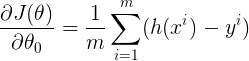
\includegraphics[scale=0.7]{{./images/eq1}} 
\end{center}

\begin{center}
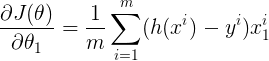
\includegraphics[scale=0.7]{{./images/eq2}} 
\end{center}

\quad Similarly, the partial derivative of the cost function w.r.t to any parameter can be denoted by 

 
\begin{center}
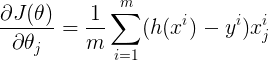
\includegraphics[scale=0.7]{{./images/eq3}} 
\end{center}

\quad We can compute the partial derivatives for all parameters at once using 

\begin{center}
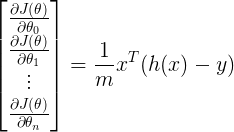
\includegraphics[scale=0.7]{{./images/eq4}} 
\end{center}

\quad where h(x) is 

\begin{center}
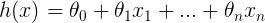
\includegraphics[scale=0.7]{{./images/eq5}} 
\end{center}

\item After computing the derivative we update the parameters as given below

\end{enumerate}
\begin{center}
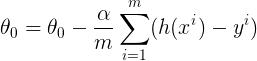
\includegraphics[scale=0.7]{{./images/eq6}} 
\end{center}

\begin{center}
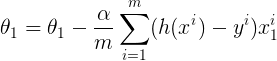
\includegraphics[scale=0.7]{{./images/eq7}} 
\end{center}

\quad where \begin{math}\alpha \end{math} is the learning parameter.

We can update all the parameters at once using, 
\begin{center}
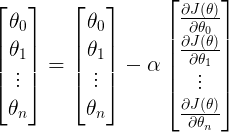
\includegraphics[scale=0.7]{{./images/eq8}} 
\end{center}

\quad We repeat the steps 2,3 until the cost function converges to the minimum value. If the value of \begin{math}\alpha \end{math}is too small, the cost function takes larger time to converge. If \begin{math}\alpha \end{math} is too large, gradient descent may overshoot the minimum and may finally fail to converge. 

\quad  To demonstrate the gradient descent algorithm, we initialize the model parameters with 0. The equation becomes Y = 0. Gradient descent algorithm now tries to update the value of the parameters so that we arrive at the best fit line. 

\newpage
\subsubsection{Python code Implementation}


\inputminted[breaklines,breakafter=d,  style=perldoc]{python}{{./pythonFile/Q_i.py}}


\subsubsection{Results}
\quad \quad The Convergence rate change for different learning rate(\begin{math}\alpha \end{math}) values are shown below.
\begin{figure}[H]
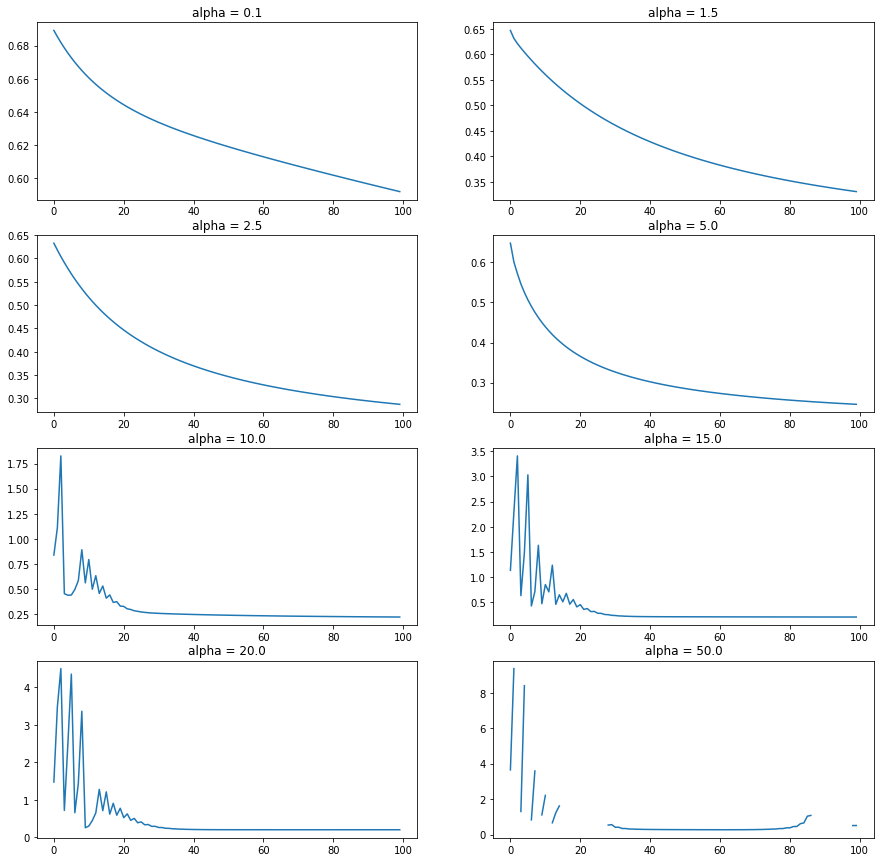
\includegraphics[width=0.8\textwidth]{{./images/Q1out}} 
\caption{Testing data output}
\end{figure}

\newpage


\subsection{LINEAR REGRESSION}
\begin{enumerate}
     \item With One Parameter
     \item With more than One Parameter 
\end{enumerate}

\subsubsection{Aim}
\quad \quad To Implement Linear Regression Model with One Parameter and with more than one parameter.


\subsubsection{Description}

\quad \quad Optimization is a big part of machine learning. Almost every machine learning algorithm has an optimization. Similarly we have for Linear regression.

\quad Linear Regression is usually the first machine learning algorithm. It is a simple model but it lays the foundation for other machine learning algorithms. It is a very powerful technique and can be used to understand the factors that influence profitability. It can be used to forecast sales in the coming months by analysing the sales data for previous months. It can also be used to gain various insights about customer behaviour. By the end of the blog we will build a model which looks like the below picture i.e, determine a line which best fits the data.

\quad The objective of a linear regression model is to find a relationship between one or more features(independent variables) and a continuous target variable(dependent variable). When there is only feature it is called Uni-variate Linear Regression and if there are multiple features, it is called Multiple Linear Regression.

\quad The linear regression model can be represented by the following equation.

\begin{center}
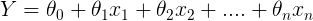
\includegraphics[scale=0.7]{{./images/eq9}} 
\end{center}

\begin{itemize}
\item Y is the predicted value
\item \begin{math} \theta_0 \end{math} is the bias term
\item \begin{math} \theta_1, \theta_2, ..., \theta_n \end{math}  are the model parameters
\item \begin{math} x_1, x_2, ..., x_n \end{math} are the feature values
\end{itemize}

\quad The above hypothesis can also be represented by 

\begin{center}
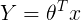
\includegraphics[scale=0.7]{{./images/eq10}} 
\end{center}

\begin{itemize}
\item  \begin{math} \theta \end{math} is the model’s parameter vector including the bias term \begin{math} \theta_0 \end{math}
\item x is the feature vector with \begin{math} x_0 = 1 \end{math}
\end{itemize}

\subsubsection{Dataset used}
\begin{enumerate}
\item With One Parameter

\quad \quad The dataset used consist of 48 data points and a single features. The feature is Production in thousands of pairs of Hosiery items. The output variable is the cost for production of these items.

\item With more than One Parameter 

\quad \quad The dataset used consist of 44 data points and two features. The features are fish weight and scale size. The output variable is the length of the fish.
\end{enumerate}

\subsubsection{Methodology To Implement This Algorithm}

\quad \quad Training of the model here means to find the parameters so that the model best fits the data. By following the procedure, we can find the best fit line for our Linear regression model. 

\quad The line for which the error between the predicted values and the observed values is minimum is called the best fit line or the regression line. These errors are also called as residuals. The residuals can be visualized by the vertical lines from the observed data value to the regression line.

\quad To define and measure the error of our model we define the cost function as the sum of the squares of the residuals. The cost function is denoted by 

\begin{center}
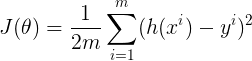
\includegraphics[scale=0.7]{{./images/eq11}} 
\end{center}

\quad where the hypothesis function h(x) is denoted by 

\begin{center}
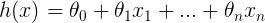
\includegraphics[scale=0.7]{{./images/eq12}} 
\end{center}

\quad and m is the total number of training examples in our data-set. 

\subsubsection{Python code Implementation}
\begin{enumerate}
\item With One Parameter

\inputminted[breaklines,breakafter=d,  style=perldoc]{python}{{./pythonFile/Q_ii_a.py}}


\newpage
\item With more than One Parameter 

\inputminted[breaklines,breakafter=d,  style=perldoc]{python}{{./pythonFile/Q_ii_b.py}}


\end{enumerate}



\subsubsection{Results}

\quad \quad Thus a Linear Regression Model with One Parameter and with more than one parameter has been implemented. The output is visible for Linear Regression with one parameter.

\begin{figure}[H]
\centering
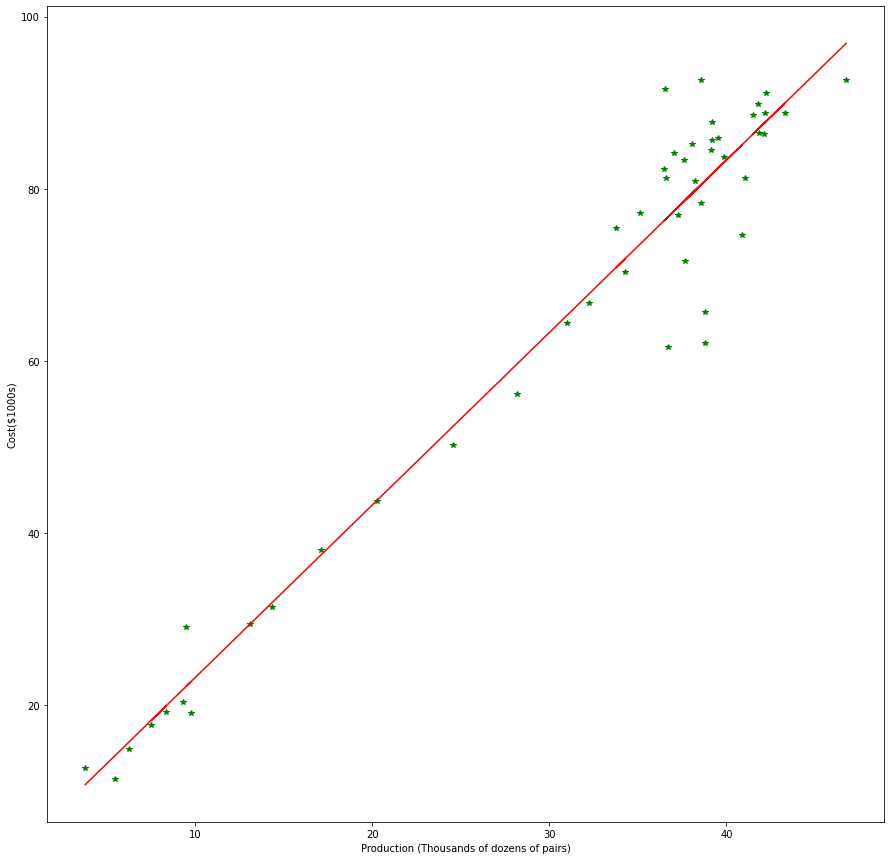
\includegraphics[width=0.5\textwidth]{{./images/Q2out}} 
\caption{Linear Regression with One parameter}
\end{figure}

\newpage



\subsection{LOGISTIC REGRESSION}

\subsubsection{Aim}
\quad \quad To Implement Logistic Regression Algorithm.


\subsubsection{Description}

\quad \quad Logistic regression is a fundamental classification technique. It belongs to the group of linear classifiers and is somewhat similar to polynomial and linear regression.

\quad Logistic regression is fast and relatively uncomplicated, and it’s convenient for you to interpret the results. Although it’s essentially a method for binary classification, it can also be applied to multi-class problems. There are 2 kinds of Logistic Regression. They are:
\begin{itemize}
    \item Single-variate logistic regression is the most straightforward case of logistic regression. There is only one independent variable (or feature), which is X = X.
    \item Multi-variate logistic regression has more than one input variable.
\end{itemize}

\subsubsection{Dataset used}

\quad \quad The dataset used consist of 100 data points and two features. The two features are exam scores in two different subject. The output variable is either 0 or 1 representing Not Getting Admitted or Getting Admitted.

\subsubsection{Methodology To Implement This Algorithm}

\quad \quad There are several general steps we taken when we’re preparing this classification model. They are: 

\begin{enumerate}
    \item Import packages, functions, and classes 
    \item Get data to work with and, if appropriate, transform it
    \item Create a classification model and train (or fit) it with your existing data 
    \item Evaluate your model to see if its performance is satisfactory 

\end{enumerate}
   
\newpage
\subsubsection{Python code Implementation}


\inputminted[breaklines,breakafter=d,  style=perldoc]{python}{{./pythonFile/Q_iii.py}}


\subsubsection{Results}

\quad \quad Thus a Logistic Regression Model has been implemented. The output is visible for Logistic Regression.

\begin{figure}[H]
\centering
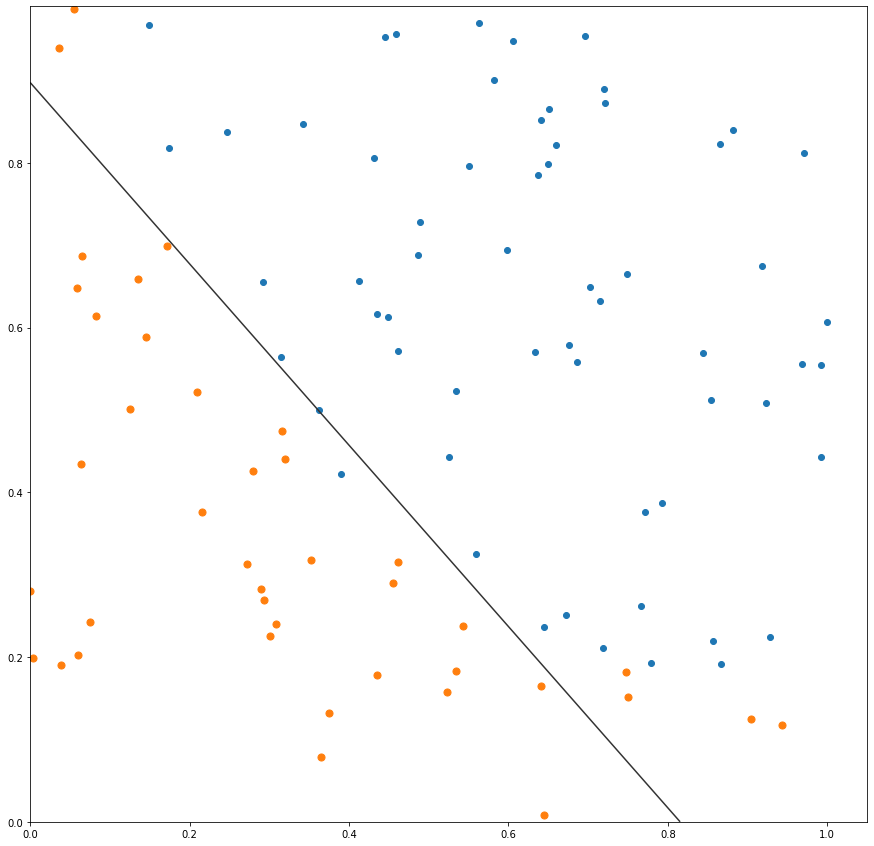
\includegraphics[width=0.7\textwidth]{{./images/Q3out}} 
\caption{Logistic Regression separating data points}
\end{figure}


\newpage




\subsection{DECISION TREES}

\subsubsection{Aim}
\quad \quad To Implement Decision trees Algorithm.


\subsubsection{Description}

\quad \quad Decision tree is one of the predictive modelling approaches used in statistics, data mining and machine learning. 

\quad A decision tree is a flowchart-like structure in which each internal node represents a test on a feature (e.g. whether a coin flip comes up heads or tails) , each leaf node represents a class label (decision taken after computing all features) and branches represent conjunctions of features that lead to those class labels. The paths from root to leaf represent classification rules 
\quad Decision trees are constructed via an algorithmic approach that identifies ways to split a data set based on different conditions. It is one of the most widely used and practical methods for supervised learning. Decision Trees are a non-parametric supervised learning method used for both classification and regression tasks. 

\quad Tree models where the target variable can take a discrete set of values are called classification trees. Decision trees where the target variable can take continuous values (typically real numbers) are called regression trees. Classification And Regression Tree (CART) is general term for this. 

 

\subsubsection{Dataset used}

\quad \quad The dataset used consist of 748 data points and four features. The features are recency of blood donation, frequency of blood donation, quantity in cc and months when blood was donated . The output variable is either 0 or 1 representing Will not donate blood or Will donate blood.

\subsubsection{Methodology To Implement This Algorithm}


\begin{itemize}
    \item Get list of rows (dataset) which are taken into consideration for making decision tree (recursively at each nodes).
    \item Calculate uncertainty of our dataset or Gini impurity or how much our data is mixed up etc.
    \item Generate list of all question which needs to be asked at that node.
    \item Partition rows into True rows and False rows based on each question asked. 
    \item Calculate information gain based on gini impurity and partition of data from previous step.
    \item Update highest information gain based on each question asked. 
    \item Update best question based on information gain (higher information gain). 
    \item Divide the node on best question. Repeat again from step 1 again until we get pure node (leaf nodes). 
\end{itemize}


\subsubsection{Python code Implementation}


\inputminted[breaklines,breakafter=d,  style=perldoc]{python}{{./pythonFile/Q_iv.py}}


\newpage

\subsubsection{Results}
\quad \quad Thus Decision Tree has been implemented. The Decision tree is visible below.

\begin{figure}[H]
\includegraphics[width=1\textwidth]{{./images/Q4Out}} 
\caption{Decision Tree}
\end{figure}

\newpage


\subsection{NAIVE BAYES ALGORITHM }

\subsubsection{Aim}
\quad \quad To Implement Naive Bayes Algorithm.


\subsubsection{Description}

\quad \quad It is a classification technique based on Bayes’ Theorem with an assumption of independence among predictors. In simple terms, a Naive Bayes classifier assumes that the presence of a particular feature in a class is unrelated to the presence of any other feature. 

\quad  Naive Bayes model is easy to build and particularly useful for very large data sets. Along with simplicity, Naive Bayes is known to outperform even highly sophisticated classification methods. Bayes theorem provides a way of calculating posterior probability P(c|x) from P(c), P(x) and P(x|c). Look at the equation below: 


\begin{center}
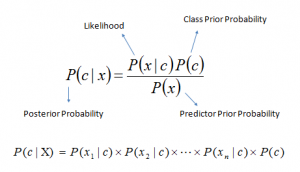
\includegraphics[scale=0.7]{{./images/eq13}} 
\end{center}

\begin{itemize}
    \item P(c$\vert$x) is the posterior probability of class (c,target) given predictor (x,attributes). 

    \item P(c) is the prior probability of class. 

    \item P(x$\vert$c) is the likelihood which is the probability of predictor given class. 

    \item P(x) is the prior probability of predictor. 

DATASET USED: 
\end{itemize}

\subsubsection{Dataset used}

\quad \quad The dataset used consist of 748 data points and four features. The features are recency of blood donation, frequency of blood donation, quantity in cc and months when blood was donated . The output variable is either 0 or 1 representing Will not donate blood or Will donate blood.

\subsubsection{Methodology To Implement This Algorithm}

\quad \quad First we will develop each piece of the algorithm in this section, then we will tie all of the elements together into a working implementation applied to a real dataset in the next section. 

\quad This Naive Bayes tutorial is broken down into 5 parts: 

\quad     Step 1: Separate By Class. 

\quad     Step 2: Summarize Dataset. 

\quad     Step 3: Summarize Data By Class. 

\quad     Step 4: Gaussian Probability Density Function. 

\quad     Step 5: Class Probabilities. 
   

\subsubsection{Python code Implementation}


\inputminted[breaklines,breakafter=d,  style=perldoc]{python}{{./pythonFile/Q_v.py}}


\subsubsection{Results}

\quad \quad Thus the Naive Bayes Algorithm has been implemented


\newpage


\subsection{RANDOM FOREST}

\subsubsection{Aim}
\quad \quad To Implement Random Forest Algorithm.


\subsubsection{Description}

\quad \quad Random forest is a supervised learning algorithm which is used for both classification as well as regression. But however, it is mainly used for classification problems. As we know that a forest is made up of trees and more trees means more robust forest. Similarly, random forest algorithm creates decision trees on data samples and then gets the prediction from each of them and finally selects the best solution by means of voting. It is an ensemble method which is better than a single decision tree because it reduces the over-fitting by averaging the result.



\subsubsection{Dataset used}

\quad \quad The dataset used consist of 748 data points and four features. The features are recency of blood donation, frequency of blood donation, quantity in cc and months when blood was donated . The output variable is either 0 or 1 representing Will not donate blood or Will donate blood.

\subsubsection{Methodology To Implement This Algorithm}

\quad \quad We can understand the working of Random Forest algorithm with the help of following steps: 

\begin{enumerate}
    \item First, start with the selection of random samples from a given dataset.
    \item Next, this algorithm will construct a decision tree for every sample. Then it will get the prediction result from every decision tree.
    \item In this step, voting will be performed for every predicted result.
    \item At last, select the most voted prediction result as the final prediction result. 
\end{enumerate}

\quad The following diagram will illustrate its working:

\begin{center}
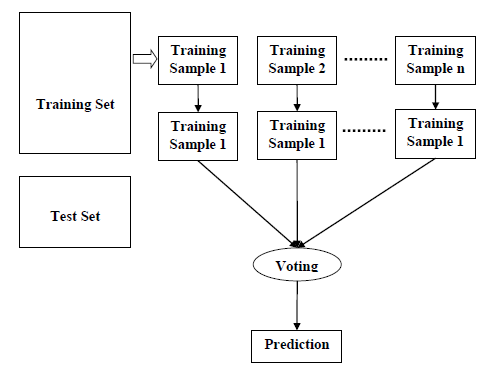
\includegraphics[scale=0.7]{{./images/pic1}} 
\end{center}


\subsubsection{Python code Implementation}


\inputminted[breaklines,breakafter=d,  style=perldoc]{python}{{./pythonFile/Q_vi.py}}


\subsubsection{Results}

\quad \quad Thus the Random Forest Algorithm has been implemented

\newpage

\subsection{ADABOOST ALGORITHM }

\subsubsection{Aim}
\quad \quad To Implement ADABOOST Algorithm.


\subsubsection{Description}

\quad \quad AdaBoost is best used to boost the performance of decision trees on binary classification problems. It was originally called AdaBoost.M1 by the authors of the technique Freund and Schapire. More recently it may be referred to as discrete AdaBoost because it is used for classification rather than regression. 

\quad AdaBoost can be used to boost the performance of any machine learning algorithm. It is best used with weak learners. These are models that achieve accuracy just above random chance on a classification problem. The most suited and therefore most common algorithm used with AdaBoost are decision trees with one level. Because these trees are so short and only contain one decision for classification, they are often called decision stumps. 

\quad Each instance in the training dataset is weighted. The initial weight is set to: 

\begin{center}
    weight(xi) = 1/n 
\end{center}

\quad Where xi is the ith training instance and n is the number of training instances.



\subsubsection{Dataset used}

\quad \quad The dataset used consist of 748 data points and four features. The features are recency of blood donation, frequency of blood donation, quantity in cc and months when blood was donated . The output variable is either 0 or 1 representing Will not donate blood or Will donate blood.

\subsubsection{Methodology To Implement This Algorithm}

\quad \quad We can understand the working of AdaBoost algorithm with the help of following steps: 

\begin{enumerate}
    \item Initially, Adaboost selects a training subset randomly. 
    \item It iteratively trains the AdaBoost machine learning model by selecting the training set based on the accurate prediction of the last training. 
    \item It assigns the higher weight to wrong classified observations so that in the next iteration these observations will get the high probability for classification. 
    \item Also, It assigns the weight to the trained classifier in each iteration according to the accuracy of the classifier. The more accurate classifier will get high weight.
    \item This process iterate until the complete training data fits without any error or until reached to the specified maximum number of estimators.
    \item     To classify, perform a "vote" across all of the learning algorithms you built. 
\end{enumerate}

\quad The following diagram will illustrate its working:

\begin{center}
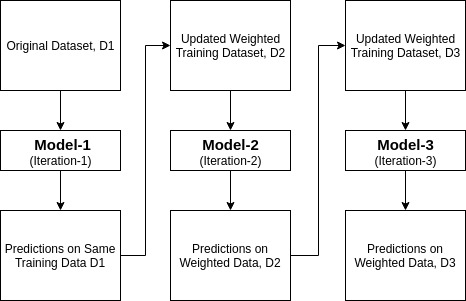
\includegraphics[scale=0.7]{{./images/pic2}} 
\end{center}

\subsubsection{Python code Implementation}


\inputminted[breaklines,breakafter=d,  style=perldoc]{python}{{./pythonFile/Q_vii.py}}


\subsubsection{Results}

\quad \quad Thus the Adaboost Algorithm has been implemented


\newpage


\subsection{SUPPORT VECTOR MACHINES }

\subsubsection{Aim}
\quad \quad To Implement Support Vector Machines Algorithm- with Linearly separable and Non- Linearly Separable cases.


\subsubsection{Description}

\quad \quad SVM is an exciting algorithm and the concepts are relatively simple. The classifier separates data points using a hyperplane with the largest amount of margin. That's why an SVM classifier is also known as a discriminative classifier. SVM finds an optimal hyperplane which helps in classifying new data points. 

\quad  In general, Support Vector Machines is considered to be a classification approach, it but can be employed in both types of classification and regression problems. It can easily handle multiple continuous and categorical variables. SVM constructs a hyperplane in multidimensional space to separate different classes. SVM generates optimal hyperplane in an iterative manner, which is used to minimize an error. The core idea of SVM is to find a maximum marginal hyperplane(MMH) that best divides the dataset into classes. 

\quad Support vectors are the data points, which are closest to the hyperplane. These points will define the separating line better by calculating margins. These points are more relevant to the construction of the classifier. 

\quad A hyperplane is a decision plane which separates between a set of objects having different class memberships. 

\quad A margin is a gap between the two lines on the closest class points. This is calculated as the perpendicular distance from the line to support vectors or closest points. If the margin is larger in between the classes, then it is considered a good margin, a smaller margin is a bad margin. 


\subsubsection{Dataset used}
\begin{enumerate}
    \item Linearly Separable
    
\quad \quad The dataset used consist of 100 data points and two features. The two features are exam scores in two different subject. The output variable is either 0 or 1 representing Not Getting Admitted or Getting Admitted.
    \item Non-Linearly Separable
    
\quad \quad The dataset used consist of 118 data points and two features. The two features are housing area and length. The output variable is either 0 or 1 representing Not sold and House being sold.

\end{enumerate}
\subsubsection{Methodology To Implement This Algorithm}

\quad \quad SVM searches for the maximum marginal hyperplane in the following steps: 

\begin{enumerate}
    \item Generate hyperplanes which segregates the classes in the best way. Left-hand side figure showing three hyperplanes black, blue and orange. Here, the blue and orange have higher classification error, but the black is separating the two classes correctly.  
    \item Select the right hyperplane with the maximum segregation from the either nearest data points as shown in the right-hand side figure. 
\end{enumerate}
 \textbf{Dealing with non-linear and inseparable planes:}

\quad In some situations like Non-linear and inseparable planes, we are unable to use, linear Separable models, then SVM uses a kernel trick to transform the input space to a higher dimensional space as shown on the right. The data points are plotted on the x-axis and z-axis (Z is the squared sum of both x and y: z=x2=y2). Now you can easily segregate these points using linear separation. 

\subsubsection{Python code Implementation}
\begin{enumerate}
    \item Linearly Separable
        
        \inputminted[breaklines,breakafter=d,  style=perldoc]{python}{{./pythonFile/Q_viii_a.py}}
        
    \item Non-Linearly Separable
     
        \inputminted[breaklines,breakafter=d,  style=perldoc]{python}{{./pythonFile/Q_viii_b.py}}
        
\end{enumerate}



\subsubsection{Results}

\quad \quad Thus the Support Vector Machines Algorithm- with Linearly separable and Non- Linearly Separable cases has been implemented

\newpage

\subsection{K-MEANS CLUSTERING }

\subsubsection{Aim}
\quad \quad To Implement K-Means Clustering Algorithm.


\subsubsection{Description}

\quad \quad K-means algorithm explores for a pre-planned number of clusters in an unlabelled multidimensional dataset, it concludes this via an easy interpretation of how an optimized cluster can be expressed.

\quad Primarily the concept would be in two steps: 
\begin{itemize}
    \item The cluster center is the arithmetic mean (AM) of all the data points associated with the cluster.
    \item Each point is adjoint to its cluster center in comparison to other cluster centers. These two interpretations are the foundation of the k-means clustering model. 
\end{itemize}
     

\quad You can take the center as a data point that outlines the means of the cluster, also it might not possibly be a member of the dataset.


\subsubsection{Dataset used}

\quad \quad The dataset used consist of 3100 data points and two features. The features are length and width of fishes.

\subsubsection{Methodology To Implement This Algorithm}

\begin{enumerate}
    \item K-centers are modeled randomly in accordance with the present value of K. 
    \item K-means assigns each data point in the dataset to the adjacent center and attempts to curtail Euclidean distance between data points. Data points are assumed to be present in the peculiar cluster as if it is nearby to center to that cluster than any other cluster center.
    \item After that, k-means determines the center by accounting the mean of all data points referred to that cluster center.It reduces the complete variance of the intra-clusters with respect to the prior step.Here, the “means” defines the average of data points and identifies a new center in the method of k-means clustering.  will get the high probability for classification. 
    \item The algorithm gets repeated among the steps 2 and 3 till some paradigm will be achieved such as the sum of distances in between data points and their respective centers are diminished, an appropriate number of iterations is attained, no variation in the value of cluster center or no change in the cluster due to data points. 
\end{enumerate}

\subsubsection{Python code Implementation}


\inputminted[breaklines,breakafter=d,  style=perldoc]{python}{{./pythonFile/Q_ix.py}}


\newpage
\subsubsection{Results}

\quad \quad Thus the K-MEANS CLUSTERING has been implemented and clustering can be seen below.


\begin{figure}[H]
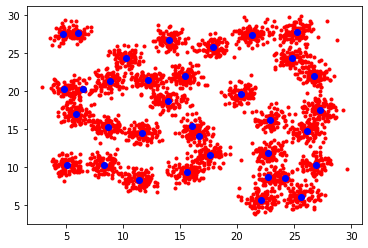
\includegraphics[width=1\textwidth]{{./images/Q9out}} 
\caption{K-means Clustering with 35 clusters}
\end{figure}


\newpage

\section{Implementation of Deeplearning Alogorithms using Tensorflow}

\subsection{AIM}
\quad \quad To write short programs in Tensor flow which uses the following objects:

\begin{enumerate}
    \item Tensorflow Constants
    \item Tensorflow Variables
    \item Tensorflow Placeholders
\end{enumerate}

\quad To write and test the back propagation algorithm using the steps of the algorithm  using Tensor Flow.

\subsection{PYTHON CODE and OUTPUT}
\begin{center}
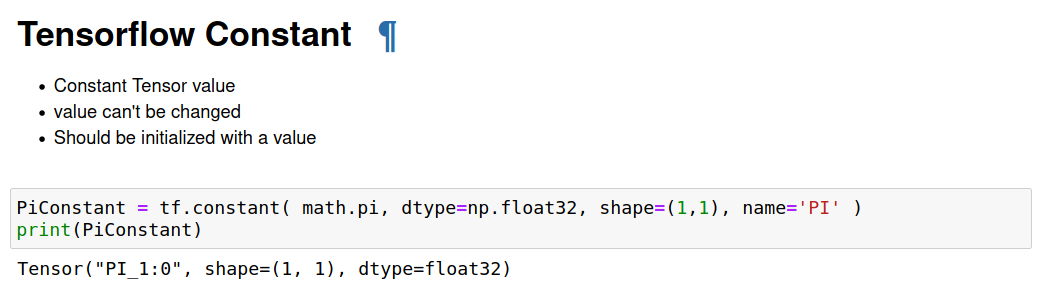
\includegraphics[scale=0.45]{{./images/TC}} 
\end{center}

\begin{center}
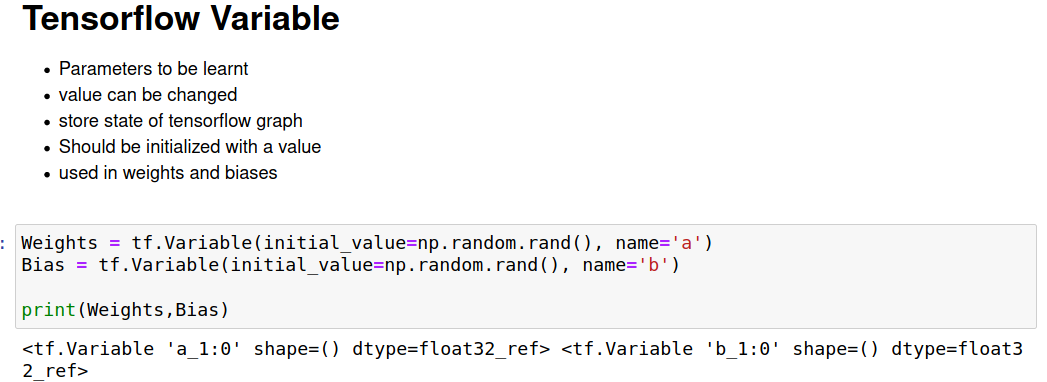
\includegraphics[scale=0.45]{{./images/TV}} 
\end{center}

\begin{center}
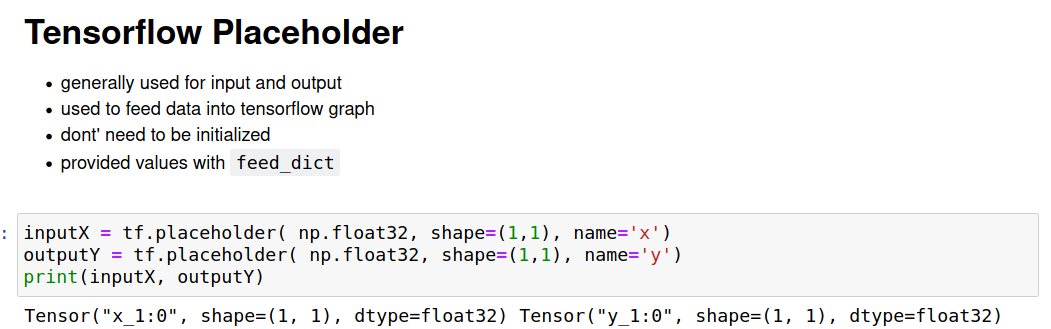
\includegraphics[scale=0.45]{{./images/TP}} 
\end{center}

\subsection{BACKPROPAGATION}

\inputminted[breaklines,breakafter=d,  style=perldoc]{python}{{./pythonFile/AIAssignment2.py}}


\newpage

\subsection{RESULT}
\quad \quad The back propagation has been implemented by tensorflow and we can observe that the error after back propagation is lesser than error before back propagation

\begin{figure}[H]
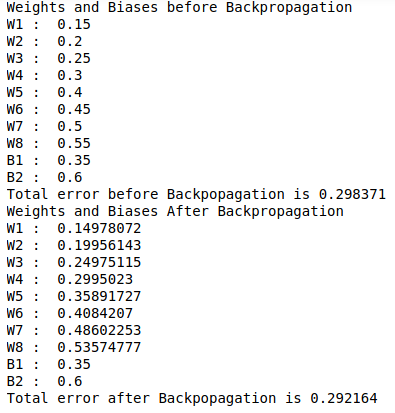
\includegraphics[width=1\textwidth]{{./images/back}} 
\caption{Back Propagation Output}
\end{figure}


\newpage
\section{Tamil Handwritten Character Recognition}

\subsection{ABSTRACT}

\quad \quad Handwritten character is constructed by executing a sequence of strokes. A structure- or shape-based representation of a stroke is used in which a stroke is represented as a string of shape features. Using this string representation, an unknown stroke is identified by comparing it with a database of strokes using a flexible string matching procedure.

\quad A full character is recognized by identifying all the component strokes. Handwritten Text Recognition is the ability of a computer to receive and interpret intelligible hand-written input from sources such as paper documents, photographs,touch-screens and other devices.

\quad A \textbf{Convolutional Neural Network (CNN)} is a Deep Learning algorithm which can take in an input image, assign importance (learnable weights and biases) to various aspects/objects in the image and be able to differentiate one from the other.

\quad The recognition of the Tamil language letters are challenging because of its various writing styles and very large number of characters. Here we wish to use CNN in recognizing handwritten Tamil characters.
\quad CNNs differ from traditional approach of Handwritten Tamil Character Recognition in extracting the features automatically and thereby increasing the chance of automation of such recognition.

\subsection{THEORY}

\quad \quad Machine simulation of human functions has been a very challenging research field since the advent of digital computers. In some areas, which entail certain amount of intelligence, such as number crunching or chess playing, tremendous improvements are achieved. 

\quad In this regard, we came across this Tamil Handwritten character Recognition. Handwritten text recognition is the ability of a machine or computer to receive and interpret handwritten text input from sources such as paper documents, photographs, Touch Screens and other devices.

\quad A handwriting recognition system handles formatting, performs correct segmentation into characters, and finds the most plausible words.  This Tamil Language had about 247 characters. \quad This creates recognition of the character is harder due to large category set and confusion between character which are similar. This makes this project to be one of the toughest handwritten recognition projects. 

\subsection{DATASET}

\quad \quad The dataset is from HP Labs India collected from native Tamil writers. There are about 156 characters with each character consisting of approximately 500 samples making the dataset about 82929 images in total.

\quad The characters used for recognition are:


\begin{center}
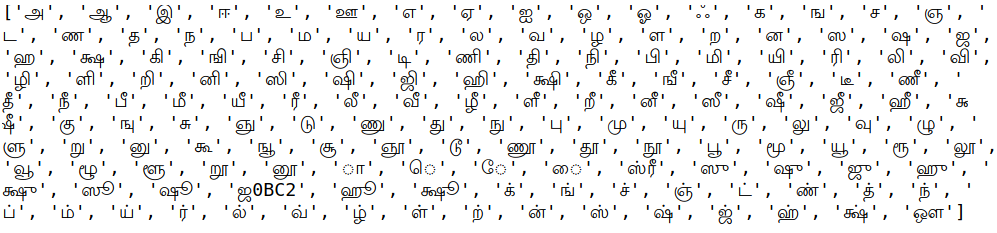
\includegraphics[scale=0.4]{{./images/tamilChar}} 
\end{center}
\subsection{METHOD USED}

\subsubsection{Pre-Processing}


\begin{itemize}
    \item In general, the images which are taken from the data set will be random resolutions. But we need to feed this data only to the CNN. So we should be able to change and resize the data according to our requirements. So we had taken the average of entire dataset, then we got the average resolution value as 128x128.
    \item Next the dataset is split into training and testing data. About 85\% of the total data i.e., 70k is given for the purpose of training the CNN Model and remaining 15\% (Approximately 13k) will be given for the testing purpose. As the splitting of data increases for the Training, the performance efficiency of the Model will increases.
    \item Here, we used One hot encoding. This allows the representation of categorical data to be more expressive. One-hot encoding ensures that machine learning does not assume that higher numbers are more important. Many machine learning algorithms cannot work with categorical data directly. The categories must be converted into numbers.
    \item The 156 character labels will be assigned to a 156x1 array. Whenever, the character is detected then that particular character’s position will be occupied by the binary bit 1, other elements positions will be represented with 0.
    \item The data set is stored as python pickle Object so as to retrieve that data without reading each and every time of simulation.
    \item Python pickle module is used for serializing and de-serializing a Python object structure. ... Pickling is a way to convert a python object (list, dictionary, etc.) into a character stream. The idea is that this character stream contains all the information necessary to reconstruct the object in another python script.
\end{itemize}

\subsubsection{Architecture}

\quad \quad The input to the CNN is 128x128 image which is passed to the architecture shown below.


\begin{figure}[H]
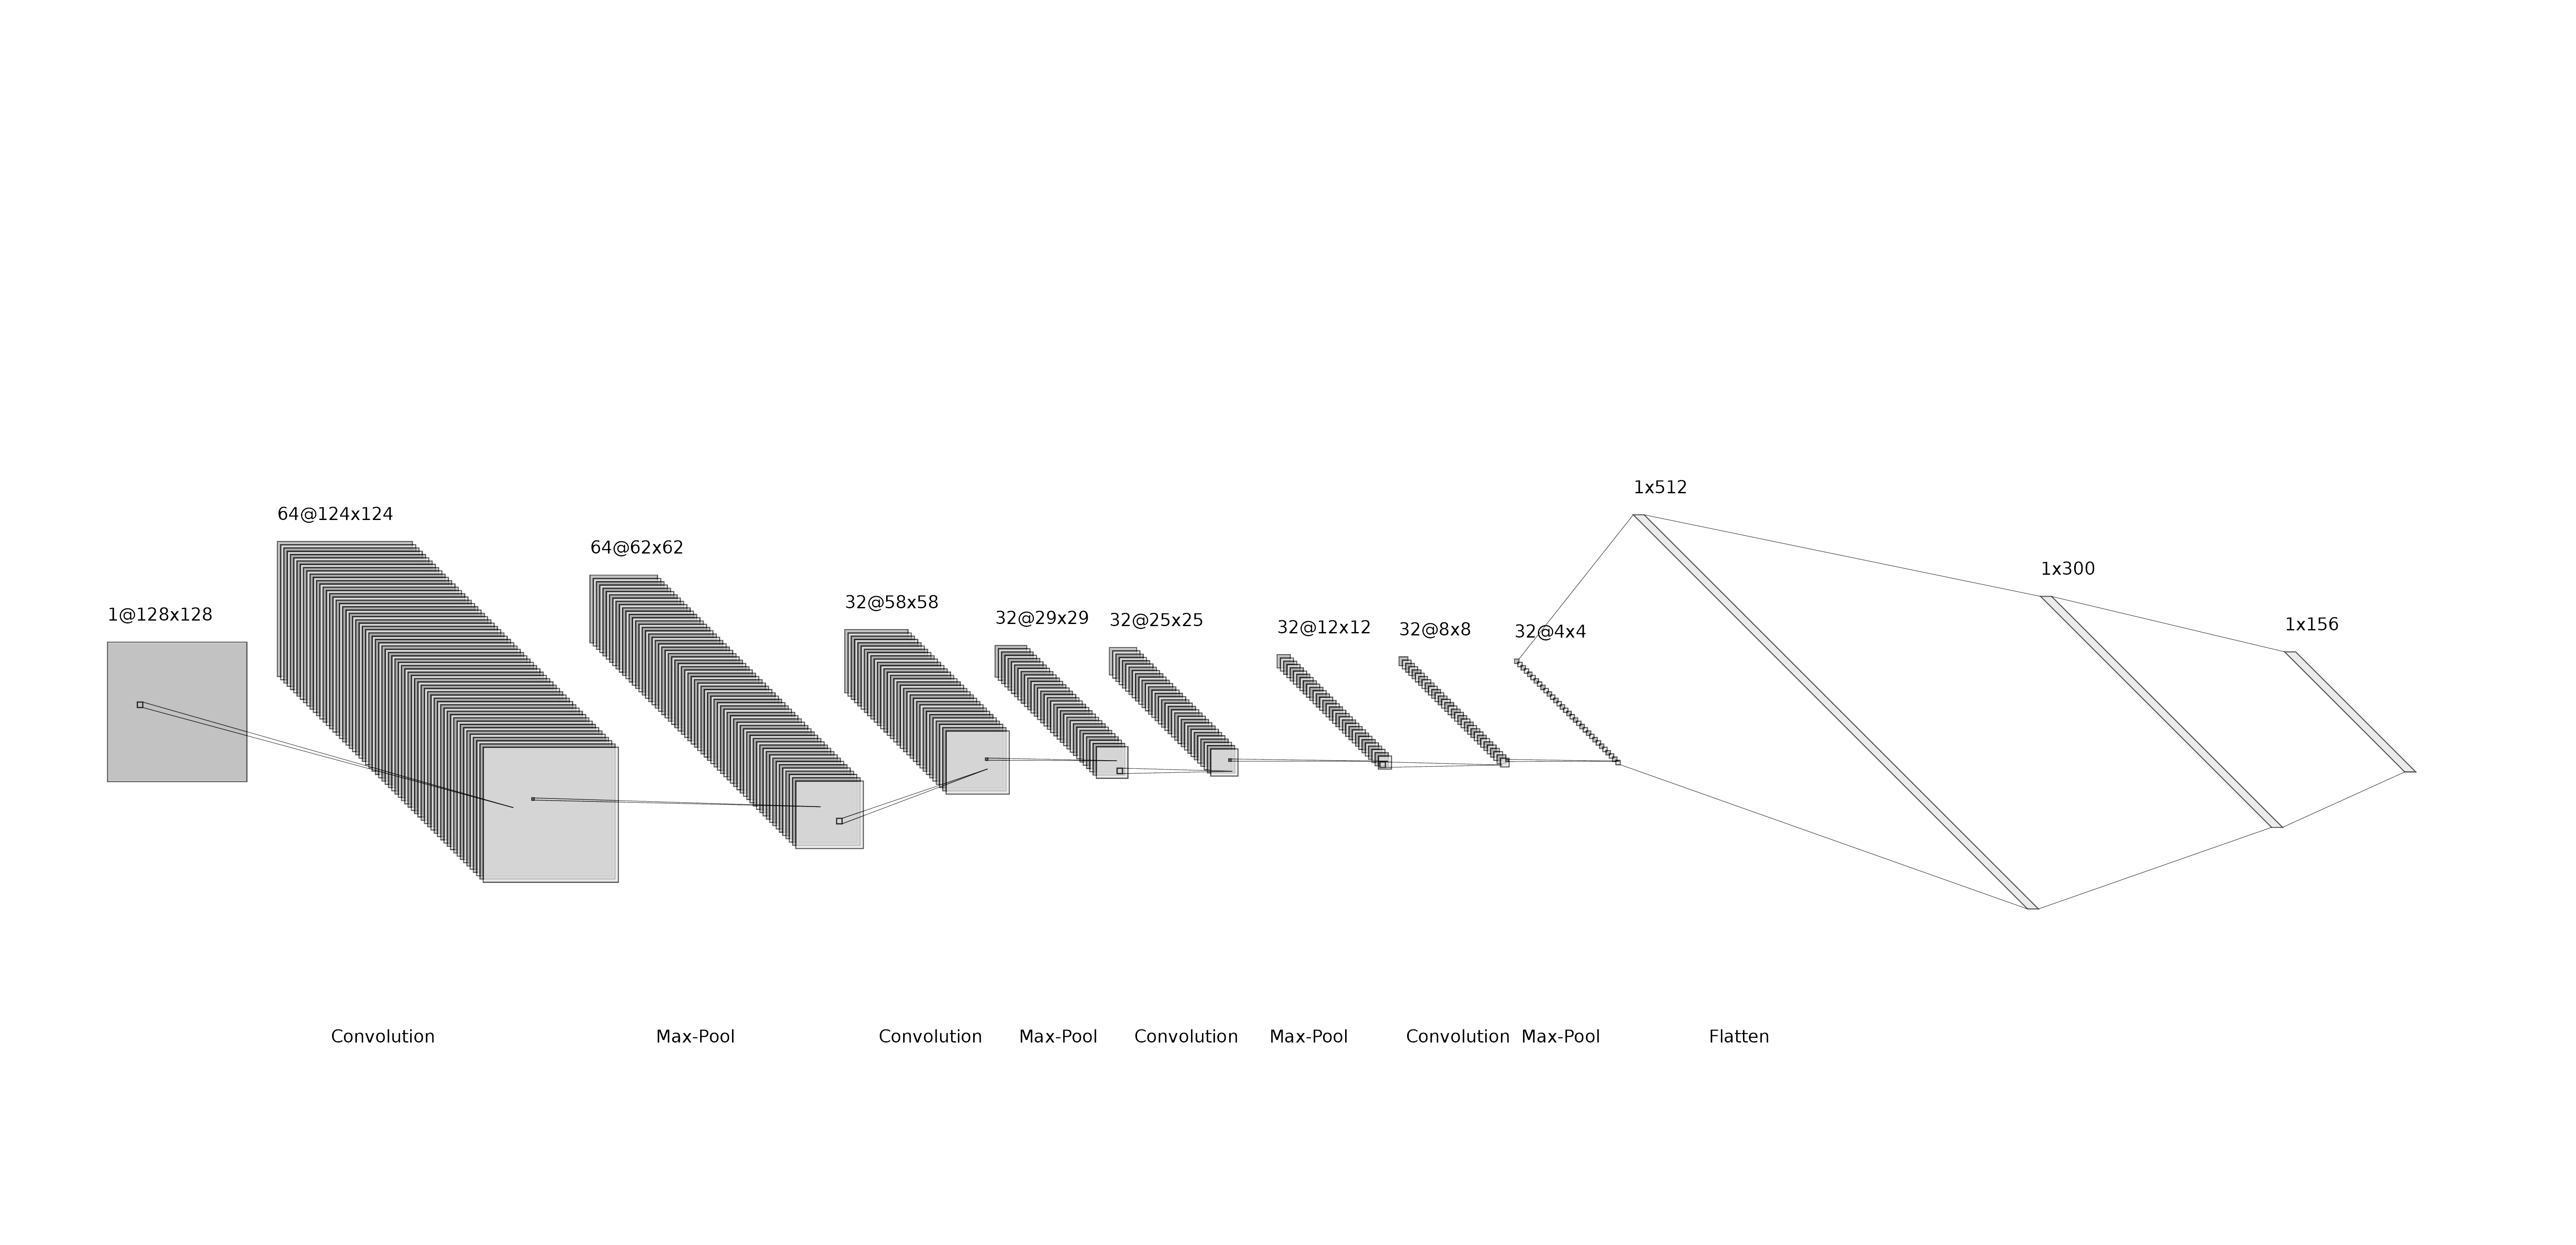
\includegraphics[width=1\textwidth]{{./images/nnn}} 
\caption{Architecture used for Tamil Handwritten character recognition}
\end{figure}


\begin{itemize}
    \item As there are 82929 images of 156 characters, which is of equal average resolution of 128x128. 
    \item This resolution of image is passed through the convolution of the particular filter, where the weight and biases which is attached with ReLU activation function learns during this process. After convolution it is passed through the max polling. During this Max. pooling operation, it calculates the max. Value in each patch of each feature map. Through this process dimension of the image decreases.
    \item Here, we pass 1@128*128 image for the convolution which gives output of 64@124*124 and after max polling it gives output of 64@62*62. We process this convolution for 4 times followed by max polling of 4 times. Finally we get 32@4*4 image which is flattening to hidden layer of 300 neurons. After that it is passed to output layer of 156 outputs.
    \item For output, we use Softmax activation function where as for convolution and hidden layer we use ReLU activation function.
\end{itemize}


\subsubsection{Brief Explanation of Architecture}

\quad We designed Our own CNN which has the following layers:-
\begin{enumerate}
    \item \textbf{Input} Images taken from the dataset, reshape. The same images used and of size 128x128x1. 
    \item \textbf{Conv-1} The first convolutional layer consists of 64 kernels of size 5x5 applied with a stride of 1 and padding of 0.
    \item \textbf{MaxPool-1} The max-pool layer following Conv-2 consists of pooling size of 2x2 and a stride of 1.
    \item \textbf{Conv-2} The second convolution layer consists of 32 kernels of size 5x5 applied with a stride of 1 and padding of 0.
    \item \textbf{MaxPool-2} The max-pool layer following Conv-2 consists of pooling size of 2x2 and a stride of 1.
    \item \textbf{Conv-3} The third conv layer consists of 32 kernels of size 5x5 applied with a stride of 1 and padding of 0.
    \item \textbf{MaxPool-3} The max-pool layer following Conv-3 consists of pooling size of 2x2 and a stride of 1.
    \item \textbf{Conv-4} The fourth conv layer consists of 32 kernels of size 5x5 applied with a stride of 1 and padding of 0.
    \item \textbf{MaxPool-4} The maxpool layer following Conv-4 consists of pooling size of 2x2 and a stride of 0.
    \item \textbf{Flattening Layer} The output of CNN is flattened to get 1x512 output.
    \item \textbf{FC-1 (Dense Layer 1)} The flattened output is fed to a hidden layer of 300 neurons.
    \item \textbf{Output (Dense Layer 2)} Finally, the output of hidden layer is fed to the output layer of 156 to get the final output.
\end{enumerate}
    
\quad All these 12 layers constitute the CNN for Tamil Hand written Character recognition Project.

\newpage

\begin{table}[H]
\resizebox{\textwidth}{!}{%
\begin{tabular}{|c|c|c|}
\hline
\textbf{Input shape} & \textbf{Layer}             & \textbf{Output shape} \\ \hline
128x128              & Convolution Layer - 64C5x5 & 124x124x64            \\ \hline
124x124x64           & MaxPooling Layer - P2x2    & 62x62x64              \\ \hline
62x62x64             & Convolution Layer - 32C5x5 & 58x58x32              \\ \hline
58x58x32             & MaxPooling Layer - P2x2    & 29x29x32              \\ \hline
29x29x32             & Convolution Layer - 32C5x5 & 25x25x32              \\ \hline
25x25x32             & MaxPooling Layer - P2x2    & 12x12x32              \\ \hline
12x12x32             & Convolution Layer - 32C5x5 & 8x8x32                \\ \hline
8x8x32               & MaxPooling Layer -  P2x2   & 4x4x32                \\ \hline
4x4x32               & Flatten Layer              & 1x512                 \\ \hline
1x512                & Hidden Layer               & 1x300                 \\ \hline
1x300                & Output Layer               & 1X156                 \\ \hline
\end{tabular}%
}
\end{table}

\quad We obtain the output shape after each layer as shown above. 

\subsubsection{Training and Testing}
\quad \quad The training is done with a total of 70,498 datas with 13 epochs. Each epochs consist of batch size of 100. The learning is done using adaptive learning rate with loss function of Categorical Cross Entropy.

\quad The testing is done on the remaining 12,440 datas from the dataset. Also, a webpage is created to test the online character recognition.

\subsection{PYTHON CODE IMPLEMENTATION}
\subsection{Preprocessing}


    \inputminted[breaklines,breakafter=d,  style=perldoc]{python}{{./pythonFile/Preprocessing.py}}


\subsection{Model Creation}

\inputminted[breaklines,breakafter=d,  style=perldoc]{python}{{./pythonFile/Cnntamil.py}}


\subsection{Online Testing using Flash APP}

\inputminted[breaklines,breakafter=d,  style=perldoc]{python}{{./pythonFile/tamilALLEzhuthukalKeras.py}}


\newpage

\subsection{RESULT}
\quad \quad The results obtained are shown below:
\begin{enumerate}
    \item Training Accuracy - 96.334%%
    \item Testing Accuracy - 91.439%%
    \item Classification Loss - 0.249
\end{enumerate}


\begin{figure}[H]
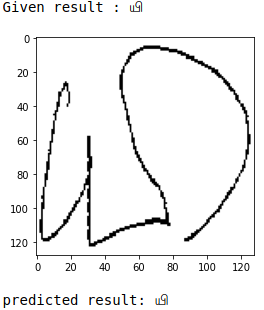
\includegraphics[width=0.8\textwidth]{{./images/cnnOut}} 
\caption{Testing data output}
\end{figure}

\begin{figure}[H]
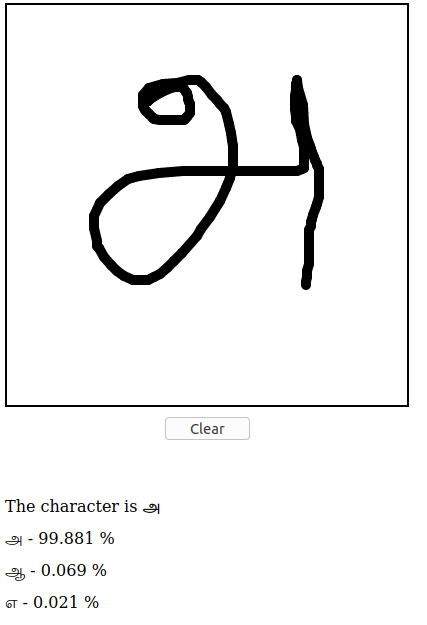
\includegraphics[width=1\textwidth]{{./images/cnnOut2}} 
\caption{Online data output}
\end{figure}


\end{document}

